%LTeX: language=it

\begin{figure}[H]
    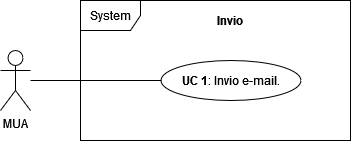
\includegraphics[width=0.55\textwidth]{sections/uc_imgs/UC-invio.png}
    \centering
    \caption{Casi d'uso relativi all'invio.}
\end{figure}

\subsection{UC 1 - Invio e-mail} \label{sec:UC1}
    
    \begin{itemize}
        \item \textbf{Attore principale}: MUA;
        \item \textbf{Descrizione}: il MUA deve poter inviare una e-mail al destinatario indicato;
        \item \textbf{Precondizioni}: l’account che il MUA gestisce è registrato nel sistema, ha una connessione aperta con il sistema ed è autenticato;
        \item \textbf{Postcondizioni}: l'e-mail è stata consegnata con successo al destinatario ed è stata salvata nel sistema;
        \item \textbf{Scenario principale}:
            \begin{enumerate}
                \item il MUA trasmette l'id dell'account (\hyperref[sec:UC1.1]{UC 1.1});
                \item il MUA trasmette l'id dell'e-mail (\hyperref[sec:UC1.2]{UC 1.2});
                \item il MUA trasmette il destinatario dell'e-mail (\hyperref[sec:UC1.3]{UC 1.3});
                \item il MUA trasmette il mittente dell'e-mail (\hyperref[sec:UC1.4]{UC 1.4});
                \item il sistema elabora l'inoltro;
            \end{enumerate}
        \item \textbf{Inclusioni}: nessuna;
        \item \textbf{Generalizzazioni}: nessuna;
        \item \textbf{Estensioni}: nessuna.
    \end{itemize}

    \begin{figure}[H]
        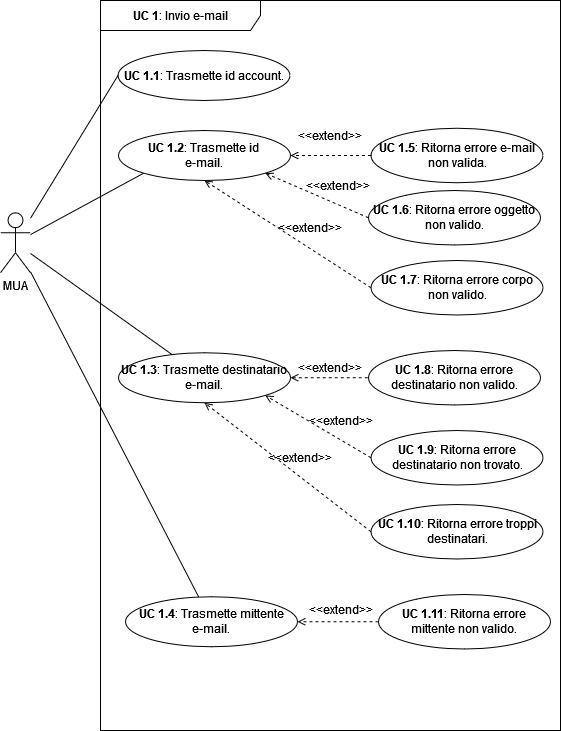
\includegraphics[width=0.85\textwidth]{sections/uc_imgs/UC01.png}
        \centering
        \caption{Diagramma sotto-casi UC 1}
    \end{figure}

    \subsubsection{UC 1.1 - Trasmette id account} \label{sec:UC1.1}
    \begin{itemize}
        \item \textbf{Attore principale}: MUA;
        \item \textbf{Descrizione}: il MUA invia al sistema l'id dell'account associato all'utente;
        \item \textbf{Precondizioni}: il MUA sta usando la funzionalità di invio di un'e-mail;
        \item \textbf{Postcondizioni}: il sistema conosce l'id dell'account;
        \item \textbf{Scenario principale}:
            \begin{enumerate}
                \item il MUA trasmette l'id dell'account associato all'utente al sistema;
            \end{enumerate}
        \item \textbf{Inclusioni}: nessuna;
        \item \textbf{Generalizzazioni}: nessuna;
        \item \textbf{Estensioni}: nessuna.
    \end{itemize}

    \subsubsection{UC 1.2 - Trasmette id e-mail} \label{sec:UC1.2}
    \begin{itemize}
        \item \textbf{Attore principale}: MUA;
        \item \textbf{Descrizione}: il MUA invia al sistema l'id dell'e-mail da inviare;
        \item \textbf{Precondizioni}: il MUA sta usando la funzionalità d'invio di un'e-mail;
        \item \textbf{Postcondizioni}: il sistema conosce l'e-mail da inviare;
        \item \textbf{Scenario principale}:
            \begin{enumerate}
                \item il MUA trasmette l'id dell'e-mail da inviare;
            \end{enumerate}
        \item \textbf{Inclusioni}: nessuna;
        \item \textbf{Generalizzazioni}: nessuna;
        \item \textbf{Estensioni}:
            \begin{enumerate}[label=\alph*.]
                \item l'e-mail non è in un formato valido:
                \begin{enumerate}[label=\arabic*.]
                    \item il sistema ritorna un errore al MUA di e-mail non valida (\hyperref[sec:UC1.5]{UC 1.5});
                \end{enumerate}
                \item l'oggetto non è in un formato valido:
                \begin{enumerate}[label=\arabic*.]
                    \item il sistema ritorna un errore al MUA di oggetto non valido (\hyperref[sec:UC1.6]{UC 1.6});
                \end{enumerate}
                \item il corpo non è in un formato valido:
                \begin{enumerate}[label=\arabic*.]
                    \item il sistema ritorna un errore al MUA di corpo non valido (\hyperref[sec:UC1.7]{UC 1.7}).
                \end{enumerate}
            \end{enumerate}
    \end{itemize}

    \subsubsection{UC 1.3 - Trasmette destinatario e-mail} \label{sec:UC1.3}
    \begin{itemize}
        \item \textbf{Attore principale}: MUA;
        \item \textbf{Descrizione}: il MUA invia al sistema il destinatario dell'e-mail;
        \item \textbf{Precondizioni}: il MUA sta usando la funzionalità d'invio di un'e-mail;
        \item \textbf{Postcondizioni}: il sistema conosce l'indirizzo di posta elettronica del destinatario dell'e-mail;
        \item \textbf{Scenario principale}:
            \begin{enumerate}
                \item il MUA trasmette il destinatario, deve soddisfare il seguente requisito:
                    \begin{itemize}
                        \item l'indirizzo e-mail deve essere sintatticamente valido;
                    \end{itemize}
            \end{enumerate}
        \item \textbf{Inclusioni}: nessuna;
        \item \textbf{Generalizzazioni}: nessuna;
        \item \textbf{Estensioni}:
            \begin{enumerate}[label=\alph*.]
                \item l'indirizzo e-mail del destinatario non è sintatticamente valido:
                \begin{enumerate}[label=\arabic*.]
                    \item il sistema ritorna un errore al MUA di destinatario non valido (\hyperref[sec:UC1.8]{UC 1.8});
                \end{enumerate}
                \item il destinatario non è stato trovato:
                \begin{enumerate}[label=\arabic*.]
                    \item il sistema ritorna un errore al MUA di destinatario non trovato (\hyperref[sec:UC1.9]{UC 1.9});
                \end{enumerate}
                \item la quantità di destinatari supera la soglia massima consentita:
                \begin{enumerate}[label=\arabic*.]
                    \item il sistema ritorna un errore al MUA di troppi destinatari (\hyperref[sec:UC1.10]{UC 1.10}).
                \end{enumerate}
            \end{enumerate}
    \end{itemize}

    \subsubsection{UC 1.4 - Trasmette mittente e-mail} \label{sec:UC1.4}
    \begin{itemize}
        \item \textbf{Attore principale}: MUA;
        \item \textbf{Descrizione}: il MUA invia al sistema il mittente dell'e-mail;
        \item \textbf{Precondizioni}: il MUA sta usando la funzionalità d'invio di un'e-mail;
        \item \textbf{Postcondizioni}: il sistema conosce l'indirizzo di posta elettronica del mittente dell'e-mail;
        \item \textbf{Scenario principale}:
            \begin{enumerate}
                \item il MUA trasmette il mittente, deve soddisfare il seguente requisito:
                    \begin{itemize}
                        \item l'indirizzo e-mail deve essere sintatticamente valido;
                    \end{itemize}
            \end{enumerate}
        \item \textbf{Inclusioni}: nessuna;
        \item \textbf{Generalizzazioni}: nessuna;
        \item \textbf{Estensioni}:
            \begin{enumerate}[label=\alph*.]
                \item l'indirizzo e-mail non è sintatticamente valido:
                \begin{enumerate}[label=\arabic*.]
                    \item il sistema invia un messaggio di errore al MUA (\hyperref[sec:UC1.11]{UC 1.11}).
                \end{enumerate}
            \end{enumerate}
    \end{itemize}

    \subsubsection{UC 1.5 - Ritorna errore e-mail non valida} \label{sec:UC1.5}
    \begin{itemize}
        \item \textbf{Attore principale}: MUA;
        \item \textbf{Descrizione}: il MUA riceve l'errore che l'e-mail non è valida;
        \item \textbf{Precondizioni}: il MUA ha trasmesso al sistema l'id dell'e-mail da inviare;
        \item \textbf{Postcondizioni}: il MUA viene notificato che l'e-mail non è valida;
        \item \textbf{Scenario principale}:
            \begin{enumerate}
                \item il sistema controlla la validità dell'e-mail e trova un errore;
            \end{enumerate}
        \item \textbf{Inclusioni}: nessuna;
        \item \textbf{Generalizzazioni}: nessuna;
        \item \textbf{Estensioni}: nessuna.
    \end{itemize}

    \subsubsection{UC 1.6 - Ritorna errore oggetto non valido} \label{sec:UC1.6}
    \begin{itemize}
        \item \textbf{Attore principale}: MUA;
        \item \textbf{Descrizione}: il MUA riceve l'errore che l'oggetto dell'e-mail non è valido;
        \item \textbf{Precondizioni}: il MUA ha trasmesso al sistema l'id dell'e-mail da inviare;
        \item \textbf{Postcondizioni}: il MUA viene notificato che l'oggetto dell'e-mail non è valido;
        \item \textbf{Scenario principale}:
            \begin{enumerate}
                \item il sistema controlla la sintassi dell'oggetto e trova un errore;
                \item il sistema notifica il MUA che l'oggetto non è valido;
            \end{enumerate}
        \item \textbf{Inclusioni}: nessuna;
        \item \textbf{Generalizzazioni}: nessuna;
        \item \textbf{Estensioni}: nessuna.
    \end{itemize}

    \subsubsection{UC 1.7 - Ritorna errore corpo non valido} \label{sec:UC1.7}
    \begin{itemize}
        \item \textbf{Attore principale}: MUA;
        \item \textbf{Descrizione}: il MUA riceve l'errore che il corpo dell'e-mail non è valido;
        \item \textbf{Precondizioni}: il MUA ha trasmesso al sistema l'id dell'e-mail da inviare;
        \item \textbf{Postcondizioni}: il MUA viene notificato che il corpo dell'e-mail da inviare non è valido;
        \item \textbf{Scenario principale}:
            \begin{enumerate}
                \item il sistema controlla la sintassi del corpo dell'e-mail e trova un errore;
                \item il sistema notifica il MUA che il corpo dell'e-mail non è valido;
            \end{enumerate}
        \item \textbf{Inclusioni}: nessuna;
        \item \textbf{Generalizzazioni}: nessuna;
        \item \textbf{Estensioni}: nessuna.
    \end{itemize}



    \subsubsection{UC 1.8 - Ritorna l'errore destinatario non valido} \label{sec:UC1.8}
    \begin{itemize}
        \item \textbf{Attore principale}: MUA;
        \item \textbf{Descrizione}: il MUA riceve l'errore che il destinatario non è valido;
        \item \textbf{Precondizioni}: il MUA ha inviato il destinatario;
        \item \textbf{Postcondizioni}: il MUA viene notificato che il destinatario non è valido;
        \item \textbf{Scenario principale}:
            \begin{enumerate}
                \item il sistema controlla la sintassi dell'e-mail del destinatario e trova un errore;
                \item il sistema notifica il MUA che il destinatario non è valido;
            \end{enumerate}
        \item \textbf{Inclusioni}: nessuna;
        \item \textbf{Generalizzazioni}: nessuna;
        \item \textbf{Estensioni}: nessuna.
    \end{itemize}


    \subsubsection{UC 1.9 - Ritorna l'errore destinatario non trovato} \label{sec:UC1.9}
    \begin{itemize}
        \item \textbf{Attore principale}: MUA;
        \item \textbf{Descrizione}: il MUA riceve l'errore che il destinatario non è stato trovato;
        \item \textbf{Precondizioni}: il MUA ha inviato il destinatario;
        \item \textbf{Postcondizioni}: il MUA viene notificato che il destinatario non è stato trovato;
        \item \textbf{Scenario principale}:
            \begin{enumerate}
                \item il sistema verifica l'esistenza del destinatario specificato;
                \item il sistema non trova il destinatario;
                \item il sistema notifica il MUA che il destinatario non è stato trovato;
            \end{enumerate}
        \item \textbf{Inclusioni}: nessuna;
        \item \textbf{Generalizzazioni}: nessuna;
        \item \textbf{Estensioni}: nessuna.
    \end{itemize}

    \subsubsection{UC 1.10 - Ritorna l'errore troppi destinatari} \label{sec:UC1.10}
    \begin{itemize}
        \item \textbf{Attore principale}: MUA;
        \item \textbf{Descrizione}: il MUA riceve l'errore che il numero dei destinatari supera la soglia massima consentita;
        \item \textbf{Precondizioni}: il MUA ha inviato i destinatari;
        \item \textbf{Postcondizioni}: il MUA viene notificato che il numero dei destinatari è eccessivo;
        \item \textbf{Scenario principale}:
            \begin{enumerate}
                \item il sistema verifica il numero di destinatari;
                \item il sistema rileva che il numero di destinatari supera la soglia massima consentita;
                \item il sistema notifica il MUA dell'eccesso di destinatari nella e-mail;
            \end{enumerate}
        \item \textbf{Inclusioni}: nessuna;
        \item \textbf{Generalizzazioni}: nessuna;
        \item \textbf{Estensioni}: nessuna.
    \end{itemize}


    \subsubsection{UC 1.11 - Ritorna l'errore mittente non valido} \label{sec:UC1.11}
    \begin{itemize}
        \item \textbf{Attore principale}: MUA;
        \item \textbf{Descrizione}: il MUA riceve l'errore che il mittente non è valido;
        \item \textbf{Precondizioni}: il MUA ha inviato il mittente;
        \item \textbf{Postcondizioni}: il MUA viene notificato che il mittente non è valido;
        \item \textbf{Scenario principale}:
            \begin{enumerate}
                \item il sistema controlla la sintassi del mittente e trova un errore;
                \item il sistema notifica il MUA che il mittente non è valido;
            \end{enumerate}
        \item \textbf{Inclusioni}: nessuna;
        \item \textbf{Generalizzazioni}: nessuna;
        \item \textbf{Estensioni}: nessuna.
    \end{itemize}



        % \subsubsection{UC 1.5 - Trasmettere gli allegati dell'e-mail} \label{sec:UC1.5}
    % \begin{itemize}
    %     \item \textbf{Attore principale}: MUA;
    %     \item \textbf{Descrizione}: il MUA invia al sistema il mittente dell'e-mail;
    %     \item \textbf{Precondizioni}: il MUA sta usando la funzionalità d'invio di un'e-mail;
    %     \item \textbf{Postcondizioni}: il sistema conosce l'indirizzo di posta elettronica del mittente dell'e-mail;
    %     \item \textbf{Scenario principale}:
    %         \begin{enumerate}
    %             \item il MUA trasmette gli allegati;
    %         \end{enumerate}
    %     \item \textbf{Inclusioni}: nessuna;
    %     \item \textbf{Generalizzazioni}: nessuna;
    %     \item \textbf{Estensioni}: 
    %         \begin{enumerate}[label=\alph*.]
    %             \item l'allegato supera la dimensione massima supporta dal sistema:
    %                 \begin{enumerate}[label=\arabic*.]
    %                     \item il sistema invia un messaggio di errore al MUA (\hyperref[sec:UC1.6]{UC 1.6}).
    %                 \end{enumerate}
    %         \end{enumerate}
    % \end{itemize}

    % \subsubsection{UC 1.8 - Ritorna l'errore massima dimensione allegati} \label{sec:UC1.8}
    % \begin{itemize}
    %     \item \textbf{Attore principale}: MUA;
    %     \item \textbf{Descrizione}: il MUA viene notificato che gli allegati dell'e-mail hanno superato la massima dimensione supportata;
    %     \item \textbf{Precondizioni}: il MUA sta usando di trasmissione degli allegati;
    %     \item \textbf{Postcondizioni}: il MUA è stato notificato del superamento della massima dimensione per gli allegati;
    %     \item \textbf{Scenario principale}:
    %         \begin{enumerate}
    %             \item il sistema controlla la dimensione degli allegati;
    %             \item il sistema nota che la dimensione è stata superata;
    %             \item il sistema notifica il MUA che la dimensione degli allegati supera la massima dimensione consentita per un e-mail;
    %         \end{enumerate}
    %     \item \textbf{Inclusioni}: nessuna;
    %     \item \textbf{Generalizzazioni}: nessuna;
    %     \item \textbf{Estensioni}: nessuna.
    % \end{itemize}